A new semi empirical method to predict roll damping has been developed as an alternative or complement to the simplified Ikeda's method. The method  predicts roll damping as a simple mathematical expression based on main particulars and does not require a hull geometry definition. 
The new method is based on regression of the present roll damping database with some additional components of Ikeda's method. Since the underlying data is collected from roll decay tests, the methods predicts the roll damping at the natural frequency $\omega_0$.  
The regression was conducted on the roll damping database for tests at even keel. 

The roll damping database reveals that the roll damping at zero speed is much lower than the roll damping at speed. The hydrodynamics at zero speed and at speed is very  different \parencite{ikeda_velocity_1979}. These two situations need to be separated so that  the regression is formulated  as a product of two sub models:
\input{equations/regression_factor_equation}
Where $B_{ehat0}$ is a zero speed regression and $B_{efactor}$ is a speed depending regression. A similar approach was used in \parencite{henry_peter_piehl_ship_2016}. Linear regression is  used for the two sub models. 

\subsection{Cross validation}
When constructing a regression model from a data set, over-fitting the data can be a problem. Including too many parameters and/or allowing too high order of the model would give a very good representation of the present roll damping data, but large extrapolation errors when the model is used on other data. Cross validation has been used to "mimic" this situation, where the model should make predictions on "new data", for ships that have not been part of the regression (the training of the model). The model that can make the best prediction on "new data" is considered as the best. The best model has been developed by optimizing the selection of parameters (the features). The regression model was allowed to have features selected from a "gross list" of all available meta data. The linear regression should determine coefficients in a mathematical expression represented as a polynomial up to second order and including coupling terms. The model with a selection of terms that gives the highest score in the cross validation is considered as the best.    

For the cross validation the data was divided into a  training set (80\%) and a testing set (20\%). The selection was made so that all tests with a specific ship model and its loading conditions were all in either the training set or the testing set. Only tests where there were results for both zero speed and speed (for the same loading condition and ship model) were included.

The "gross list" of available features has been chosen as a balance between guessed relevance and to minimize the number of tests that need to be excluded due to missing meta data. 
The number of parameters was also kept to a minimum so that a set of fewer features was selected prior to one with more features if they had similar scoring. As it turned out the developed regression models (equation \ref{eq:polynom_zero} and \ref{eq:polynom_speed}) have no coupling terms or quadratic terms.

The total regression model, consisting of the two sub models, was evaluated using cross validation. 100 random train/test sets were fitted and tested giving an average score: $mean(R^2)=0.68$, with standard deviation $std(R^2)=0.12$.

Figure \ref{fig:B_e_hat0_regression} and \ref{fig:B_e_factor_regression} shows comparisons between the regressions and the corresponding model test data. It can be noted that the speed factor can be up to 3.5 so that the roll damping at speed is 3.5 times larger than the corresponding roll damping at zero speed. The regressed sub models are shown in equation \ref{eq:polynom_zero} and \ref{eq:polynom_speed}. The non-dimensional damping due to hull lift $B_{LHAT}$, from the Ikeda method, is one of the parameters in the speed dependency equation \ref{eq:polynom_speed}. A comparison for the total regression model (equation \ref{eq:regression_factor_equation}) is shown in figure \ref{fig:B_e_factor_regression_total}, where it can be noticed that the error does not have the same ship draught dependence as the simplified method has. 

\begin{equation} \label{eq:polynom_zero}
B_{e hat 0} = - 0.0136 A_{0} + 0.759 BK_{B} + 0.0726 GM - 0.0303 T + 0.00126 \omega_{0 hat} + 0.0143
\end{equation}

\begin{equation} \label{eq:polynom_speed}
B_{e hat} = 363.359008235359 B_{L HAT} - 0.134270511572716 I_{RUD} - 8.20659228064392 OG + 1.12171452657267 V - 20.0713800117644 kg + 2.05991359954373
\end{equation}

{\footnotesize \underline{Note}: All input parameters are normalized using Froude scaling with $L_{pp}$ as scale factor. $\omega_{0hat}$ is non-dimensional according to \parencite{himeno_prediction_1981}.} 

\begin{figure}[H]
\centering
\begin{minipage}{.5\textwidth}
  \centering
  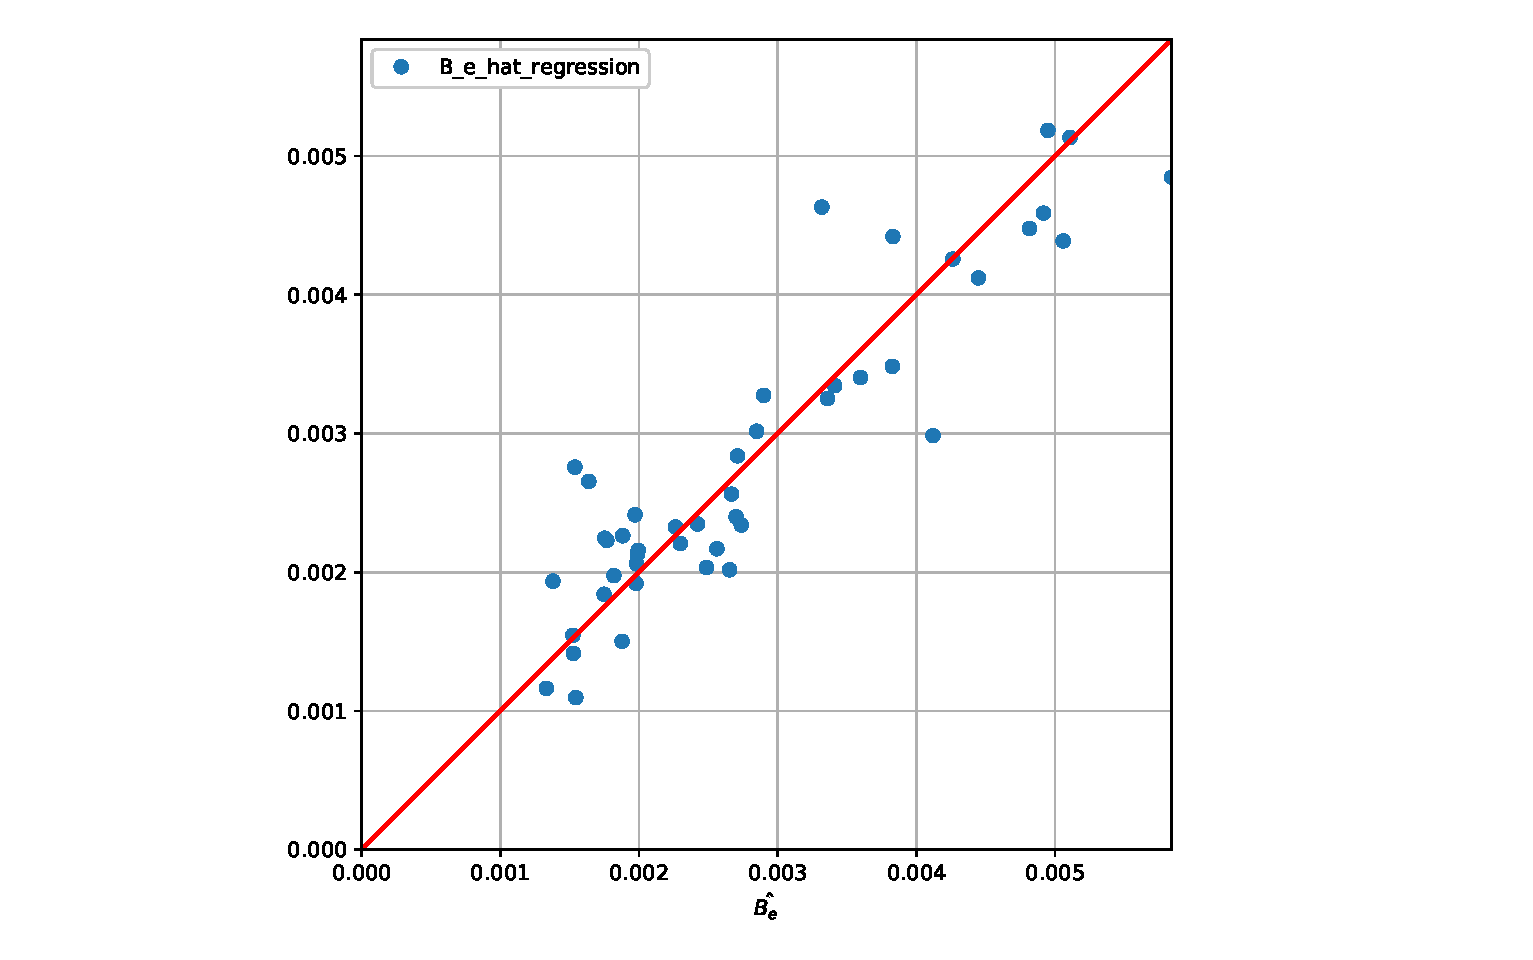
\includegraphics[width=\columnwidth]{figures/B_e_hat0_regression.eps}
    \caption{Comparison between predictions with the zero speed model and the damping at zero speed from the database}
    \label{fig:B_e_hat0_regression}
\end{minipage}%
\begin{minipage}{.5\textwidth}
  \centering
 \includegraphics[width=\columnwidth]{figures/B_e_factor_regression.eps}
    \caption{Speed dependency regression}
    \label{fig:B_e_factor_regression}
\end{minipage}
\end{figure}


\begin{figure}[H]
    \centering
    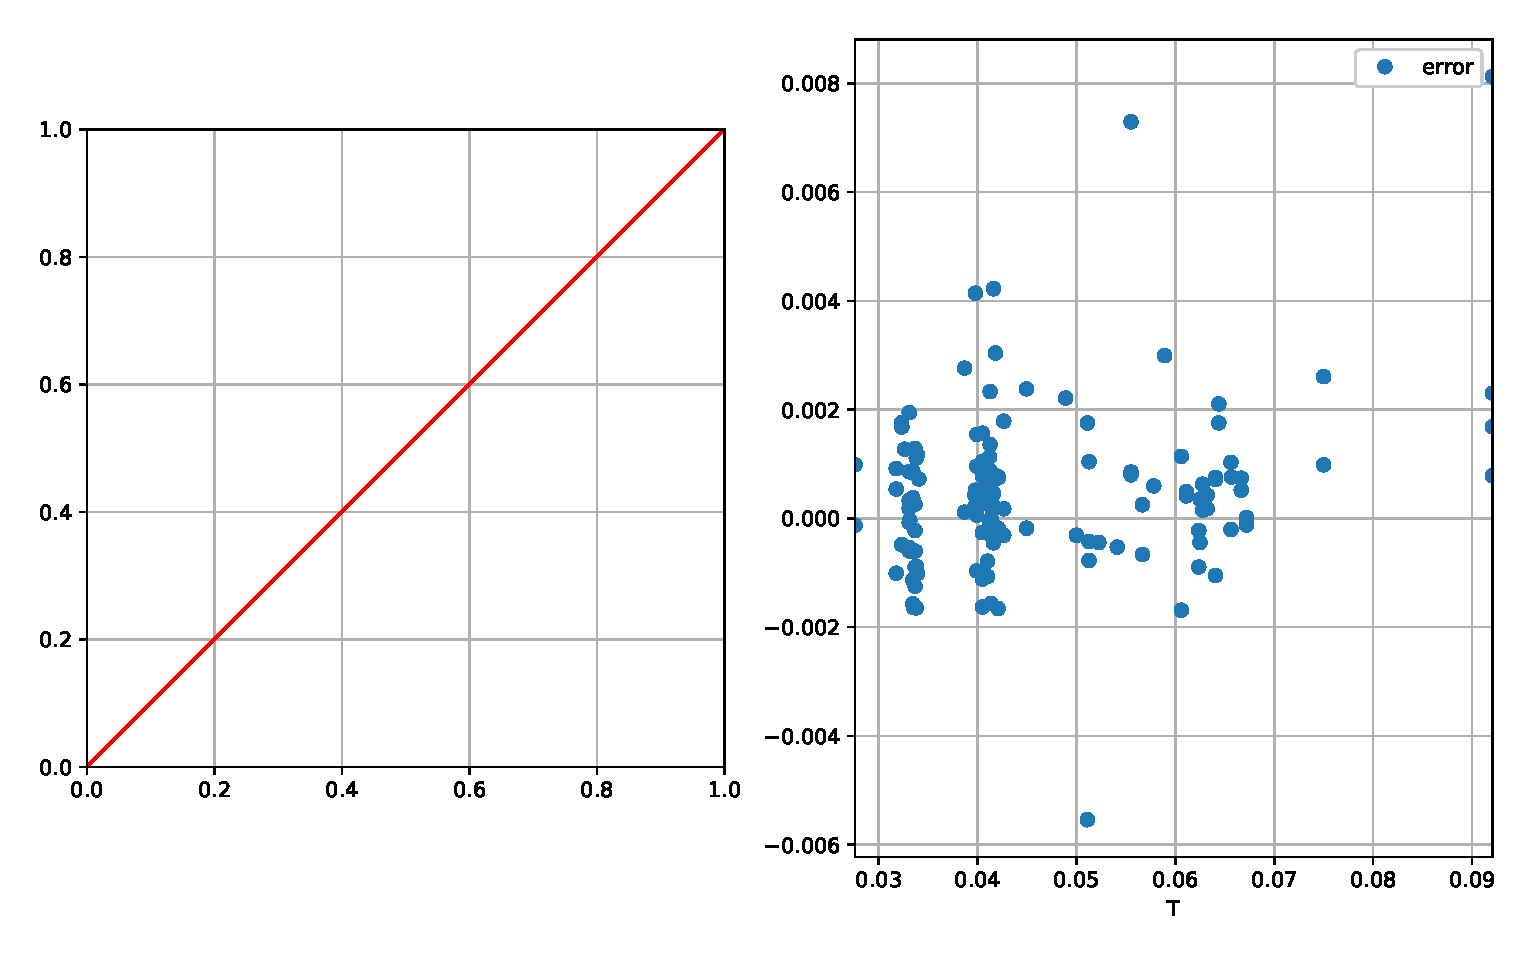
\includegraphics[width=\columnwidth]{figures/B_e_factor_regression_total.eps}
    \caption{Total regression}
    \label{fig:B_e_factor_regression_total}
\end{figure}
